\section{Aufgabe1}
\label{sec:Aufgabe1}
%\lstinputlisting[language=Python, firstline=2, lastline=67]{plots/aufgabe1.py}
\subsection{a)}
Teilaufgabe a) befindet sich auf den abgegebenen Zetteln.
\label{subsec:a}

\subsection{b)}
\label{subsec:b}
\begin{figure}[H]
  \centering
  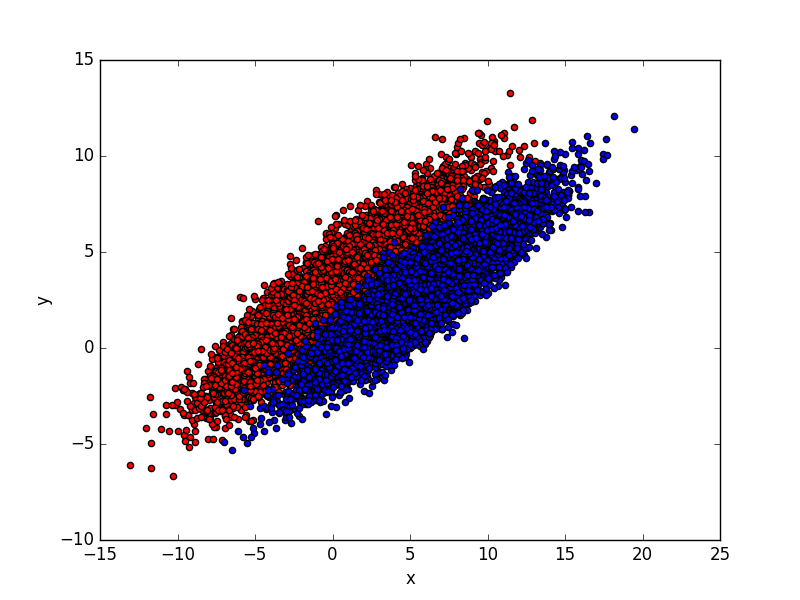
\includegraphics[width=\textwidth]{plots/scatterplot.png}
  \caption{Scatterplot der beiden Populationen P\_0 und P\_1.}
  \label{fig:scatterplot}
\end{figure}

\subsection{c)}
Um die Korrellation $\rho$ zu berechnen wurde folgende Formel benutzt.
\begin{equation}
  \rho = \frac{\sigma_{xx} \cdot \sigma_{yy}}{\sigma_{xy}}
  \label{eqn:rho}
\end{equation}
\label{subsec:c}
\begin{table}[H]
  \centering
  \caption{Mithilfe des Codes errechnete Werte.}
  \label{tab:Werte}
  \begin{tabular}{c|c|c|c|c|c|c}
            &$\mu_x$&$\mu_y$&$\sigma_{xx}^2$&$\sigma_{yy}^2$&Kovarianz $\sigma_{xy}=\sigma_{yx}$&\rho\\
            \hline
Population 1&0.0029 & 2.9818& 11.921        & 6.430         & 7.915                            1.10&\\
Population 2&6.0153 & 3.1254& 12.207        & 5.406         & 7.340                            1.11&\\
Gesamt      &3.0091 & 3.0536& 21.101        & 5.922         & 7.843                            1.43&\\
  \end{tabular}
\end{table}
